% RESULTS
%   - Show the unbounded Queue Graph and the mess it makes of LB and GM
%   - Show soft ECVN allows more work to be done, possibly at the cost of accumulating K.
%   - Shwo that HARD ecn allows the best operation -- work gets done and less K is accumlated.

% Show a control. 
% Normal operation. Highlight the bursty peaks from the \ac{DGI} algorithm running
% Point out the average queue size as a second line.
% State a relationship between the average queue size and the message delay.

% Introduce a sufficent amount of traffic to make the queue drain off slowly, recreating the previous figure
% State again that as the amount of other traffic increases the time to drain the queue starts to increase
% State that this does not affect normal operation because the \ac{DGI} has slack built into the schedule to ensure that a normal amount of background traffic does not cripple the \ac{DGI}.
% State that as the traffic increases further, eventually it will over flow the queue
% Show the unbounded queue growth for a drop tail queue.

% Introduce the \ac{RED} queue.
% Show that the \ac{RED} queue, without notifying the \ac{DGI} can do some management, but it isn't sufficent to keep the groups together.
% Show that based on the control, less work gets done and the groups change more frequently.

% Introduce the \ac{ECN} notification
% If the \ac{RED} queue allows \ac{DGI} traffic to pass (making the \ac{RED} queue more like a drop-tail for \ac{DGI} traffic) show that it improves on the previous scenario.
% Show that however, eventually the traffic reaches a threshold where the stratedgy is not sufficent to prevent issues.
% Introduce the \ac{DGI} reacting to the notifications.
% Show that when the \ac{DGI} goes into a maintain mode the average traffic drops.
% Show that this allows a large group to be maintained and the migrations to proceed as normal (with the time reduced schedule).

% Introduce HARD groupbreaks.
% Show that a hard group break greatly reduces traffic (even more than previously) & that this allows the \ac{DGI} to determine how to split.
% Demonstrate a worst-case scenario where the group break is not optimal.
% Show that a planned hard break allows that group to continue operating.

\section{Results}
\label{sect:results}
Figures \ref{fig:plota} and \ref{fig:plotb} show the normal operation of the system.
In this configuration, there is no congestion on the network. 
The \ac{DGI}s start, group together and then begin migrating power between processes.
Figure \ref{fig:plota} plots the queue size over time for a queue used to send packets from a switch to the router.
Figure \ref{fig:plotb} is a detailed view of a portion of Figure \ref{fig:plota}.
Figure \ref{fig:plotb} shows the queue size during the normal operation of group management as well as the first migration of the load balancing module.
The dotted line plots the \ac{EWMA} of the size of the queue.

\begin{figure}
\centering
\adjustbox{valign=t}{
\begin{minipage}{.48\linewidth}
\centering
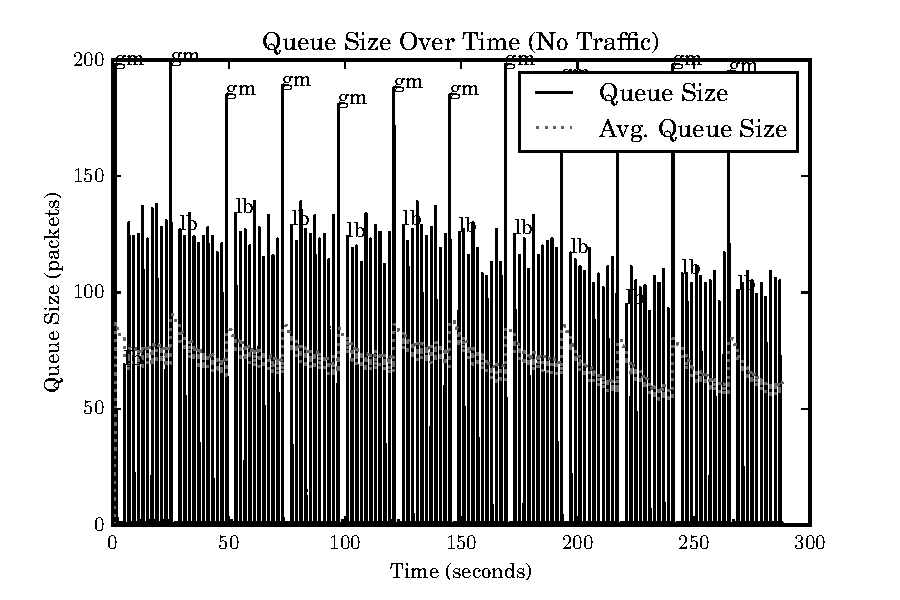
\includegraphics[width=\textwidth]{a-qsizeot-notraffic-all.pdf}
\caption{Plot of the queue size for a queue from switch A to the router when only the DGI generates traffic.}
\label{fig:plota}
\end{minipage}}%
\hfill
\adjustbox{valign=t}{
\begin{minipage}{.48\linewidth}
\centering
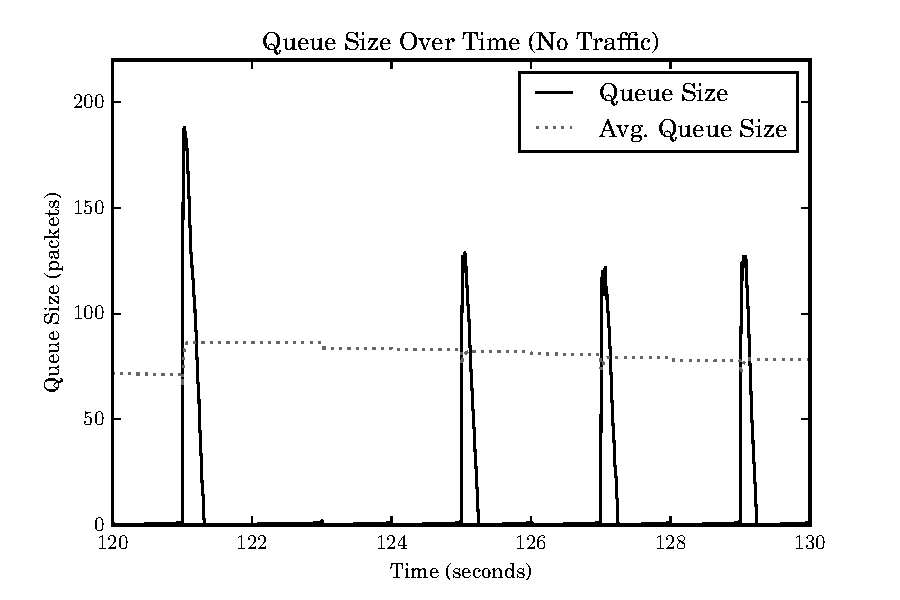
\includegraphics[width=\textwidth]{b-qsizeot-notraffic-120s-130s.pdf}
\caption{Detailed view of Figure \ref{fig:plota}. The left most peak is from Group Management, and the 3 smaller peaks are from power migrations.}
\label{fig:plotb}
\end{minipage}}
\end{figure}

\begin{figure}
\centering
\adjustbox{valign=t}{
\begin{minipage}{.48\linewidth}
\centering
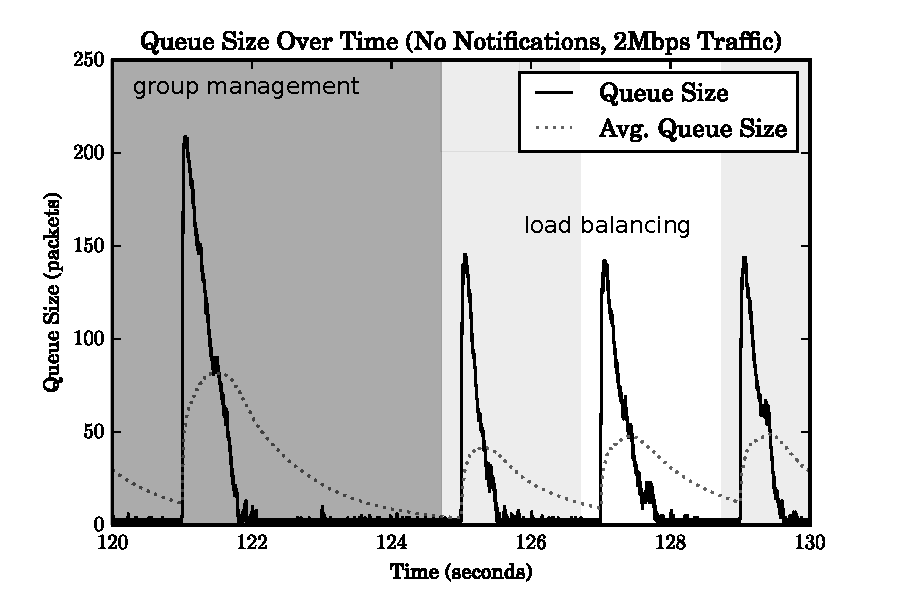
\includegraphics[width=\textwidth]{e-qsizeot-nonotifications-2mbpstraffic-120s-130s.pdf}
\caption{Detailed view of the effect on queue size as other network traffic is introduced. Compared to Figure \ref{fig:plotb}, the peaks are taller and wider. Background traffic causes the average queue size to be updated more frequently.}
\label{fig:plote}
\end{minipage}}%
\hfill
\adjustbox{valign=t}{
\begin{minipage}{.48\linewidth}
\centering
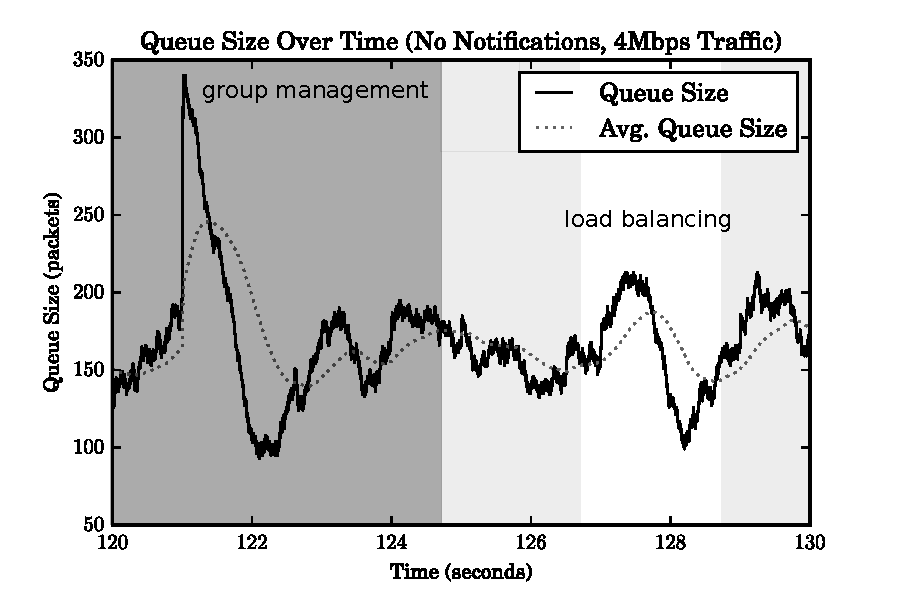
\includegraphics[width=\textwidth]{f-qsizeot-nonotifications-4mbpstraffic-120s-130s.pdf}
\caption{Detailed view of the effect on queue size as other network traffic is introduced. With no \ac{ECN} notifications, the peak from Group Management is much larger. The congestion is sufficient that the Group Management and Load Balancing modules are affected.}
\label{fig:plotf}
\end{minipage}}%
\end{figure}

%From this experiment we establish the $min_{th}$ value used as a \ac{RED} queue parameter.
%The traffic generated by each step of the group management algorithm is very bursty.
%It should be obvious that the tightness of the clock synchronization in the group affect how large this peak is.
%Figure \ref{fig:plotc} plots the power level of the processes in the system.
%Like \cite{HILTESTBED}, the level of the power at a process is the net sum of its power generation capability and load.
%As power is shared on the network, processes with excess generation, converge toward zero net power.
%Demand processes also converge toward zero net power.
%The number of migrations completed is a good metric for how much work can be performed.
%Figure \ref{fig:plotc} represents NUMBER migrations between the 30 processes used in the control.

\begin{figure}
\centering
\adjustbox{valign=t}{
\begin{minipage}{.48\linewidth}
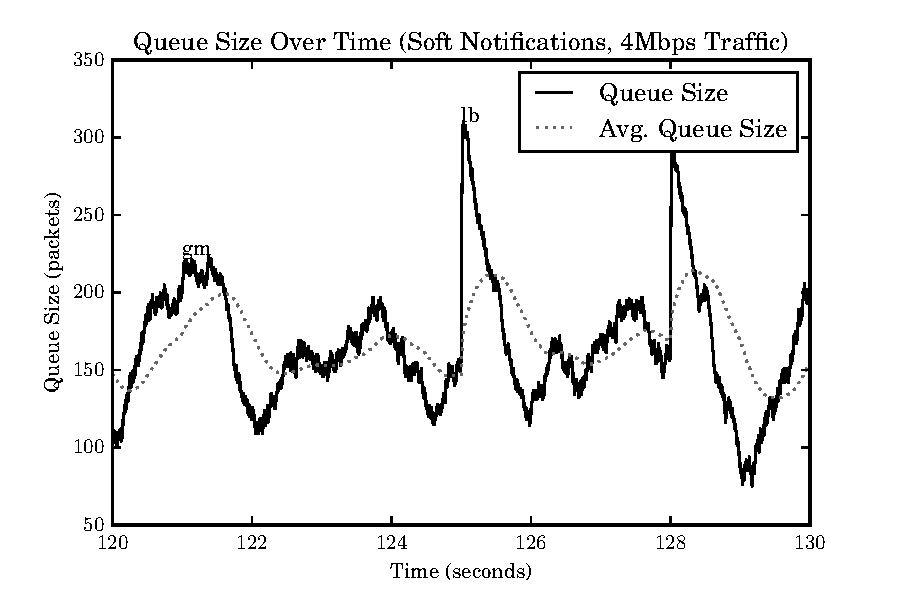
\includegraphics[width=\textwidth]{i-qsizeot-softnotifications-4mbpstraffic-120s-130s.pdf}
\caption{Detailed view of the effect on queue size as other network traffic is introduced. In this scenario, the ECN notifications put Group Management into a maintenance mode that reduces its message complexity and switches Load Balancing to slower migration schedule, preventing undesirable behavior.}
\label{fig:ploti}
\end{minipage}}%
\hfill
\adjustbox{valign=t}{
\begin{minipage}{.48\linewidth}
\centering
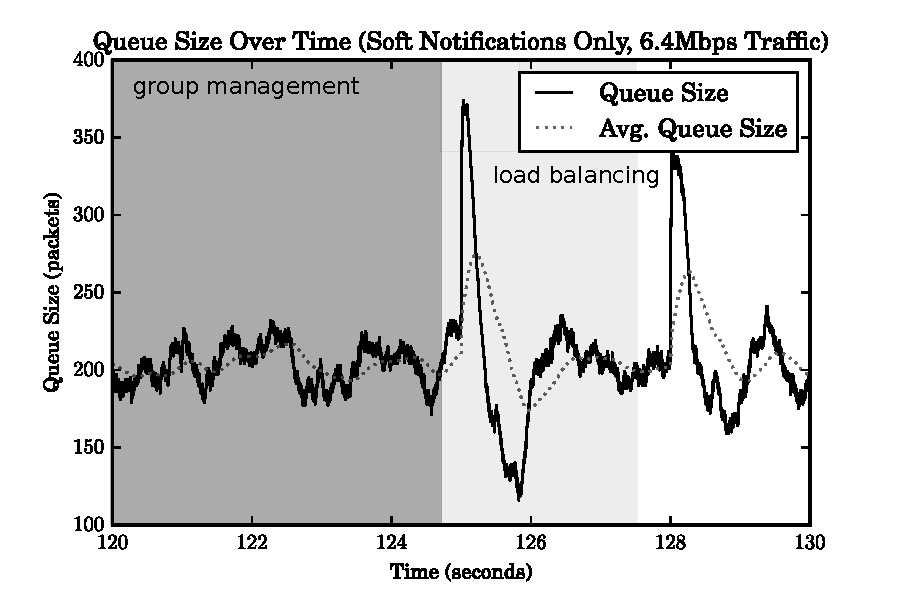
\includegraphics[width=\textwidth]{k-qsizeot-softnotificationsonly-64mbpstraffic-120s-130s.pdf}
\caption{Detailed view of the effect on queue size as a large amount network traffic is introduced. Groups are unstable and processes occasionally leave the main group. Some migrations are lost due to queueing delays.}
\label{fig:plotk}
\centering
\end{minipage}}
\end{figure}

\begin{figure}
\centering
\adjustbox{valign=t}{
\begin{minipage}{.48\linewidth}
\centering
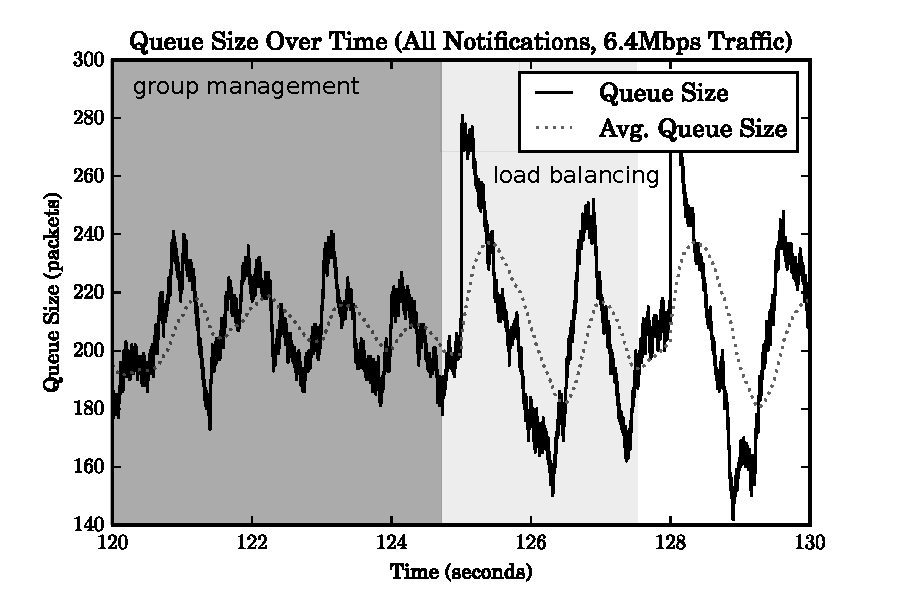
\includegraphics[width=\textwidth]{l-qsizeot-allnotifications-64mbpstraffic-120s-130s.pdf}
\caption{Effect on queue size as a large amount of network traffic is introduced. Hard notifications cause the groups to divide. As a result of the smaller groups, the group management and load balancing peaks are smaller than those in \ref{fig:plotk}. No migrations are lost.}
\label{fig:plotl}
\end{minipage}}%
\hfill
\adjustbox{valign=t}{
\begin{minipage}{.48\linewidth}
\centering
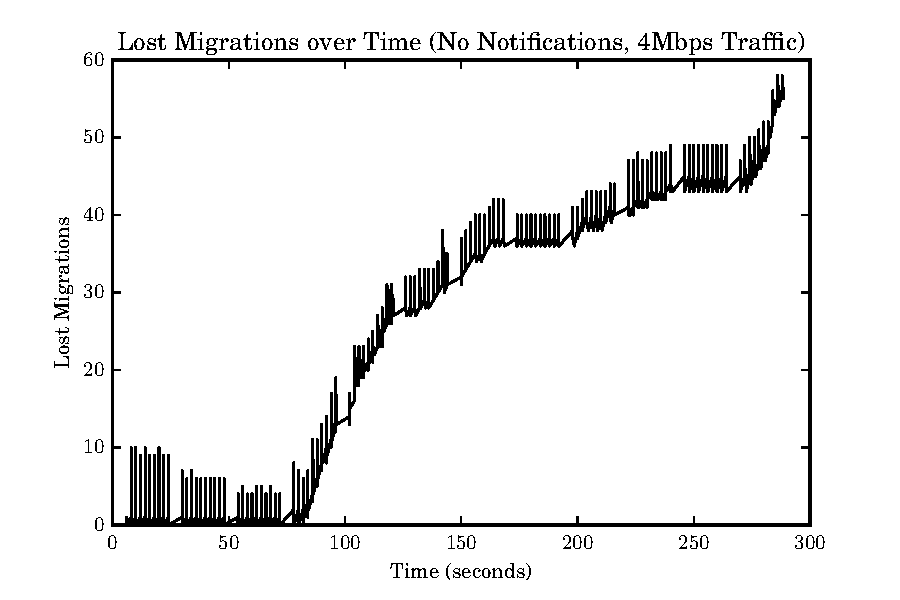
\includegraphics[width=\textwidth]{g-lostm-nonotifications-4mbpstraffic-all.pdf}
\caption{Count of lost migrations from all processes over time. Migrations are counted as lost until the second process confirms it has been completed. Without congestion management, a large number of migrations are lost.}
\label{fig:plotg}
\end{minipage}}
\end{figure}

Figure \ref{fig:plote} shows the queue size as the network traffic begins to increase.
The \ac{DGI}s in these experiments use a schedule that allows for some congestion to occur before processes are disrupted.
This slack gives the network devices the opportunity to identify when the network congestion will go beyond the acceptable threshold.

Figure \ref{fig:plotf} shows an example of congestion affecting the physical network without \ac{ECN}.
As a result of the congestion in Figure \ref{fig:plotf}, processes leave the main group.
Additionally power migrations are affected: migrations are lost, or the supply process is left uncertain of migrations completions.
Figure \ref{fig:plotg} plots the count of failed migrations over time.
%In this scenario, only XXX migrations are completed compared to the control.

Figure \ref{fig:ploti} shows an example of the \ac{ECN} algorithm notifying processes of the congestion.
Compared to the scenario in Figure \ref{fig:plotf}, the \ac{ECN} algorithm successfully prevents the group from dividing, and increases the number of migrations by reducing the number of attempted migrations each round.

Figures \ref{fig:plotl} and \ref{fig:plotk} show an example of a more extreme congestion scenario.
In Figure \ref{fig:plotl}, the \ac{RED} algorithm shares a Hard \ac{ECN} notification.
This notification causes the \ac{DGI} to switch to a smaller fallback configuration.
This fallback configuration decreases the queue usage from Figure \ref{fig:plotk} to Figure \ref{fig:plotl}.
Without this fallback configuration behavior, the system is greatly affected by the traffic.
However, with the fallback configuration the system remains stable and no migrations are lost.

%Table X summarizes the number of migrations and number of failed migrations for each of the presented scenarios.
